% !TeX spellcheck = de_DE
\section{\ExercisePrefixEmbeddedC DHT11 \optional}

\optionaltextbox

Der DHT11 ist ein Temperatur- und Feuchtigkeitssensor, der mithilfe des Steckplatine an den Microcontroller angeschlossen werden kann.
Der DHT11 hat 4 Anschlüsse (Pins), von denen im Rahmen des Praktikums 3 verwendet werden.
Zwei Pins werden für Masse (\lstinline|GND|) und Versorgungsspannung (\lstinline|VCC|) genutzt und ein Pin für die digitale Datenübertragung zwischen dem DHT11 und dem Microcontroller.
Abbildung \ref{fig:dht11Pins} zeigt die Pin-Belegung des DHT11.
Pin 1 wird mit \lstinline|VCC| verbunden und Pin 4 mit \lstinline|GND|.
Pin 2 ist ein I/O-Pin zur digitalen Datenübertragung.
In dieser Aufgabe ist es das Ziel die Temperatur- und Feuchtigkeitswerte des Sensors kontinuierlich auszulesen und diese auf dem Display darzustellen.
\begin{figure}[!htb]
	\centering
	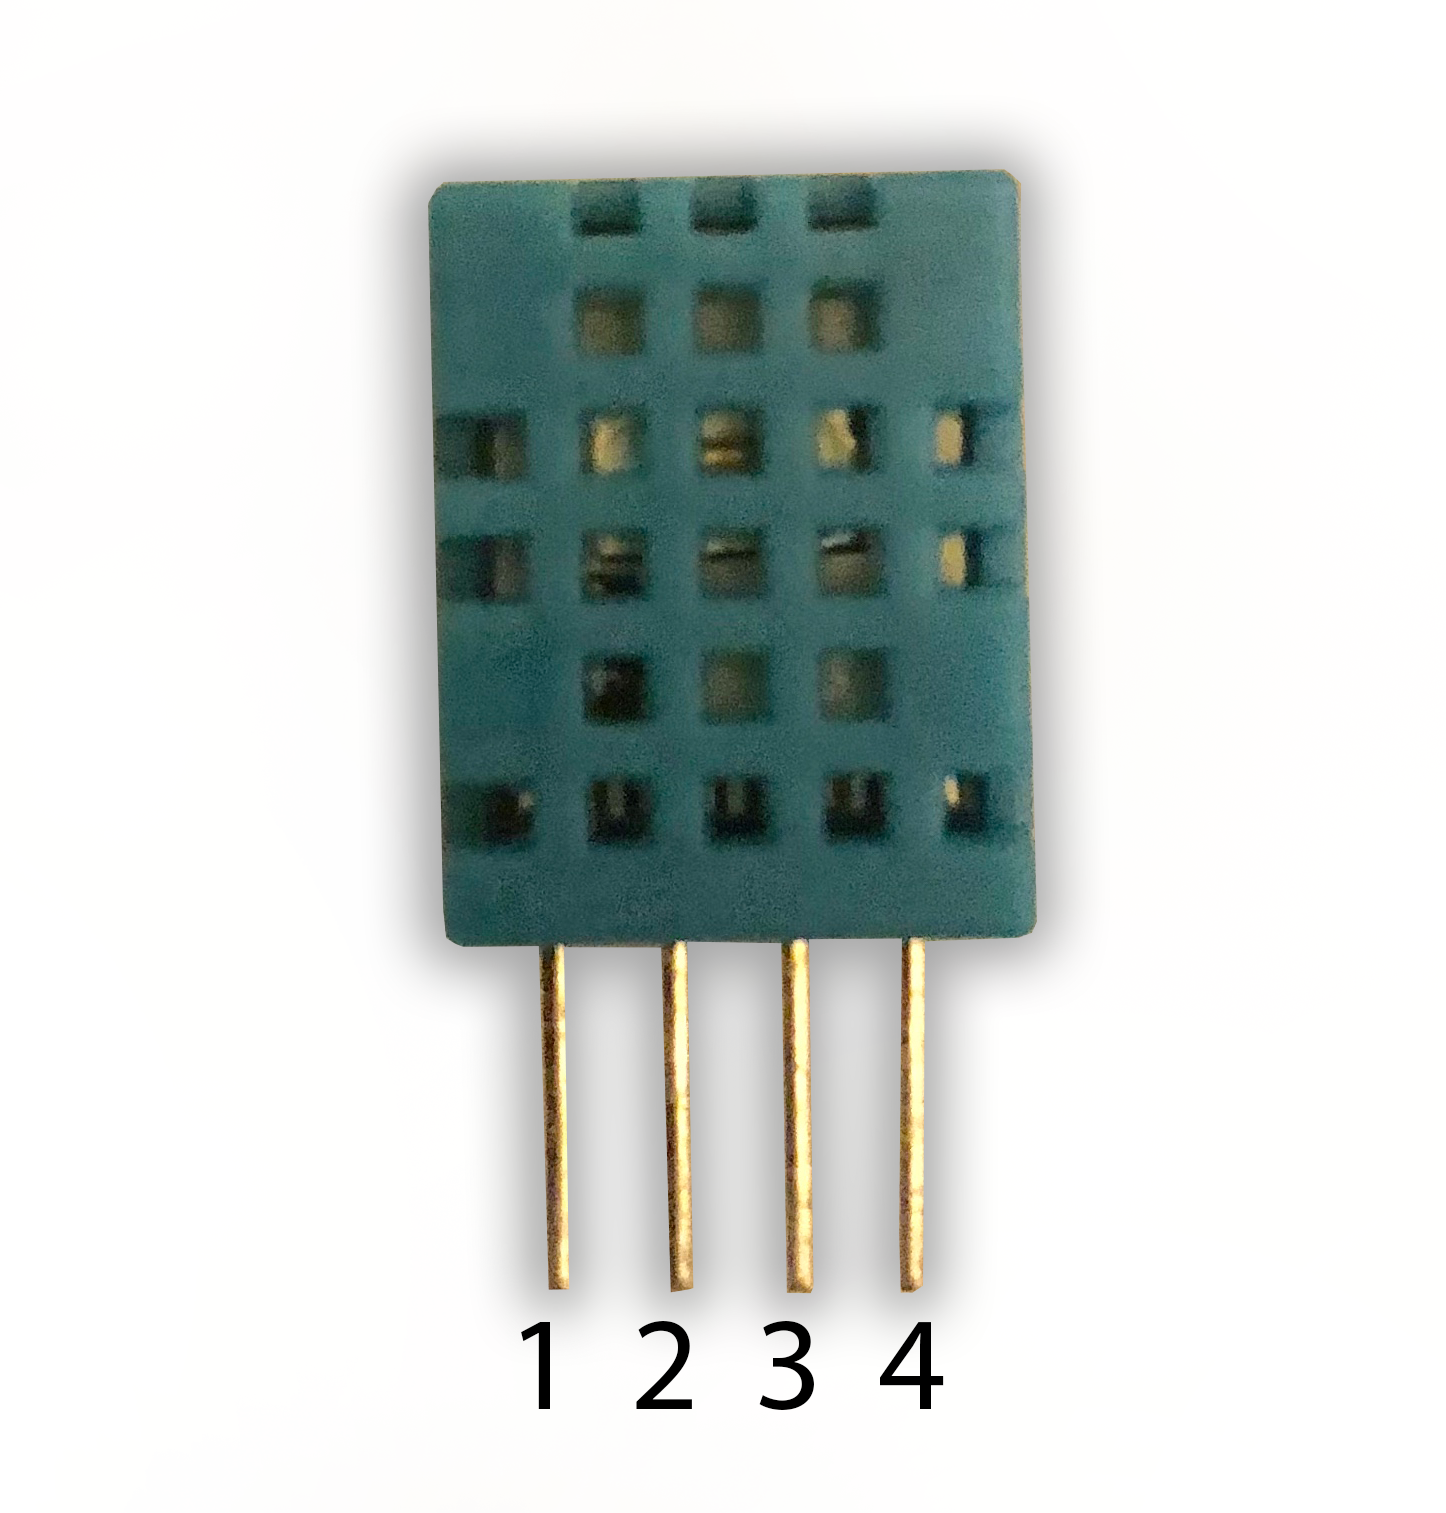
\includegraphics[width=0.2\textwidth]{./05_c/figures/DHT11.png}
	\caption{DHT11 Pinbelegung}
	\label{fig:dht11Pins}
\end{figure} 

\begin{enumerate}
\item 
Zunächst trenne den Microcontroller von der Stromzufuhr und stelle sicher, dass dieser ausgeschaltet ist.
Verbinde gemäß Abbildung \ref{fig:dht11Schematics} den DHT11 mit dem Microcontroller.
Der DHT11 wird, von links gezählt, an den dritten Pin des CN17 Steckers des Microcontrollers angeschlossen (Port 5, Pin 2, Präprozessorkonstante \lstinline|GPIO1PIN_PF52|).
Nutze als Unterstützung Abbildung~\ref{fig:cpppWiring}, die schematisch die GPIO-Verbindungen des Microcontrollers darstellt.
Bevor der Microcontroller wieder an den Computer angeschlossen wird, lasse die Verkabelung von einem Tutor überprüfen.
%
\begin{figure}[!htb]
	\centering
	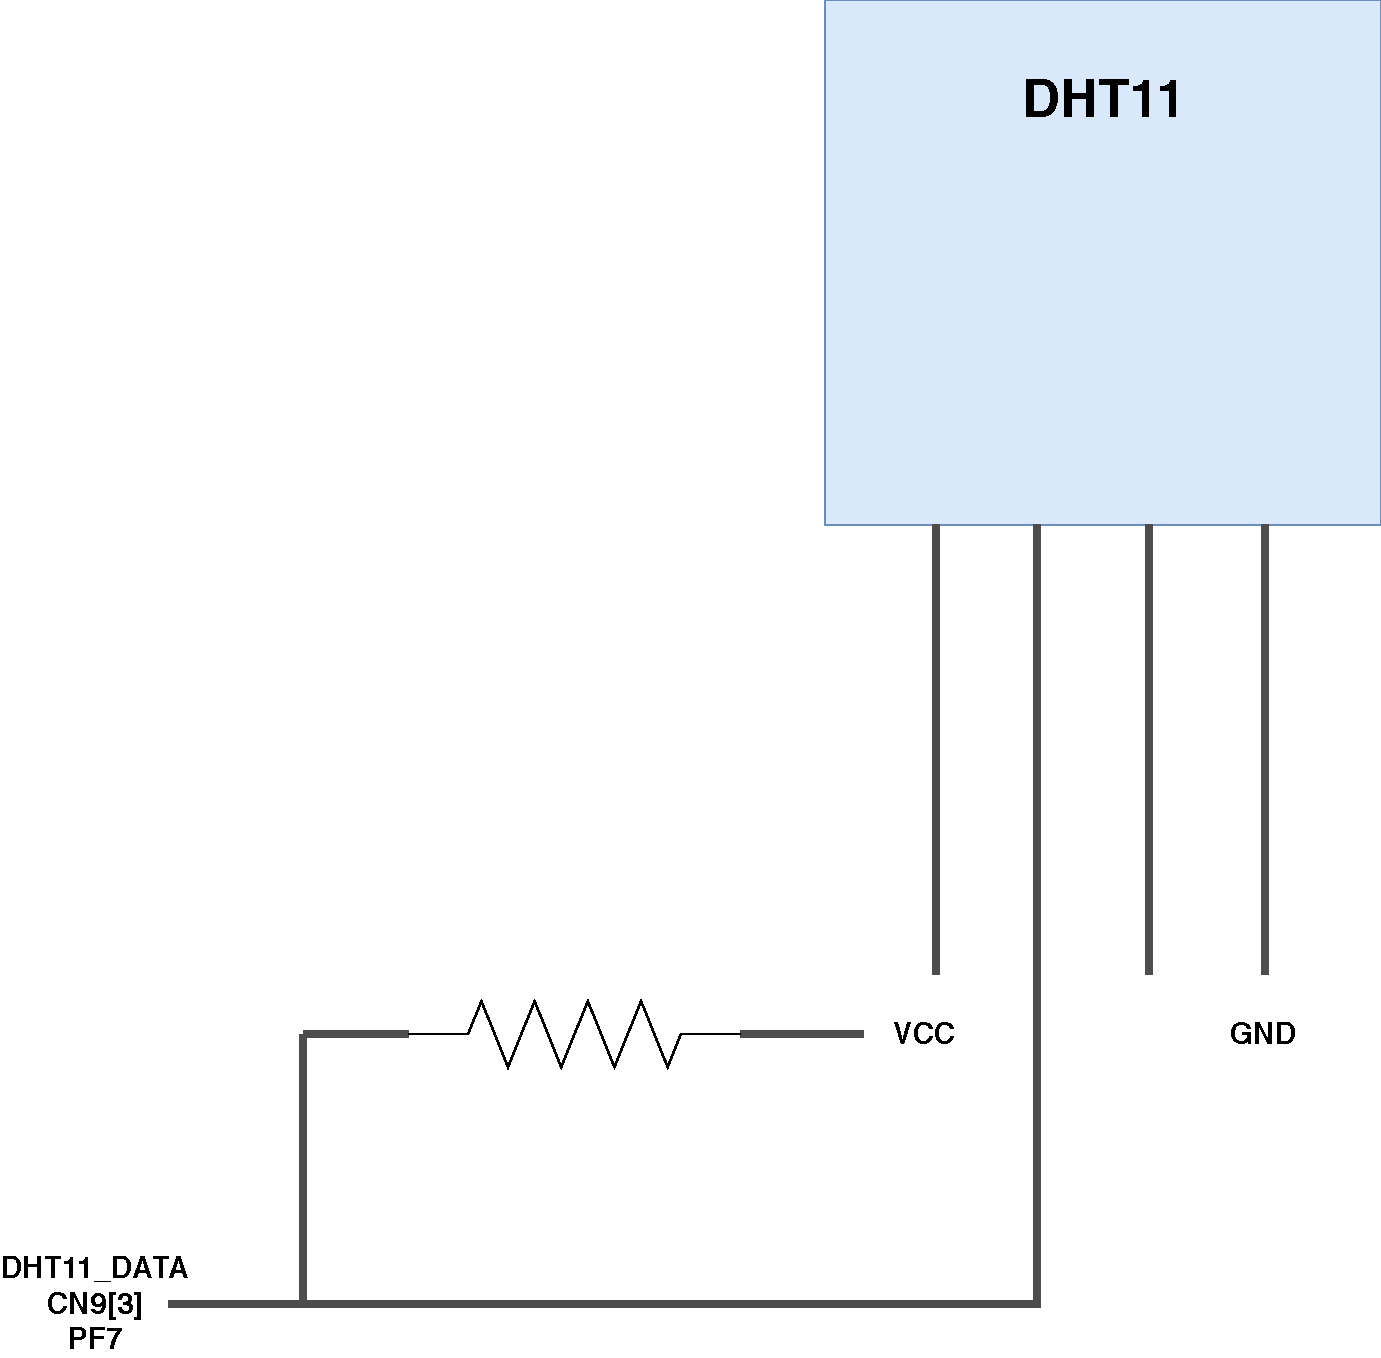
\includegraphics[width=0.35\textwidth]{./05_c/figures/DHT11-Schematics.pdf}
	\caption{Verkabelung des DHT11}
	\label{fig:dht11Schematics}
\end{figure} 
\begin{figure}[!htb]
	\centering
	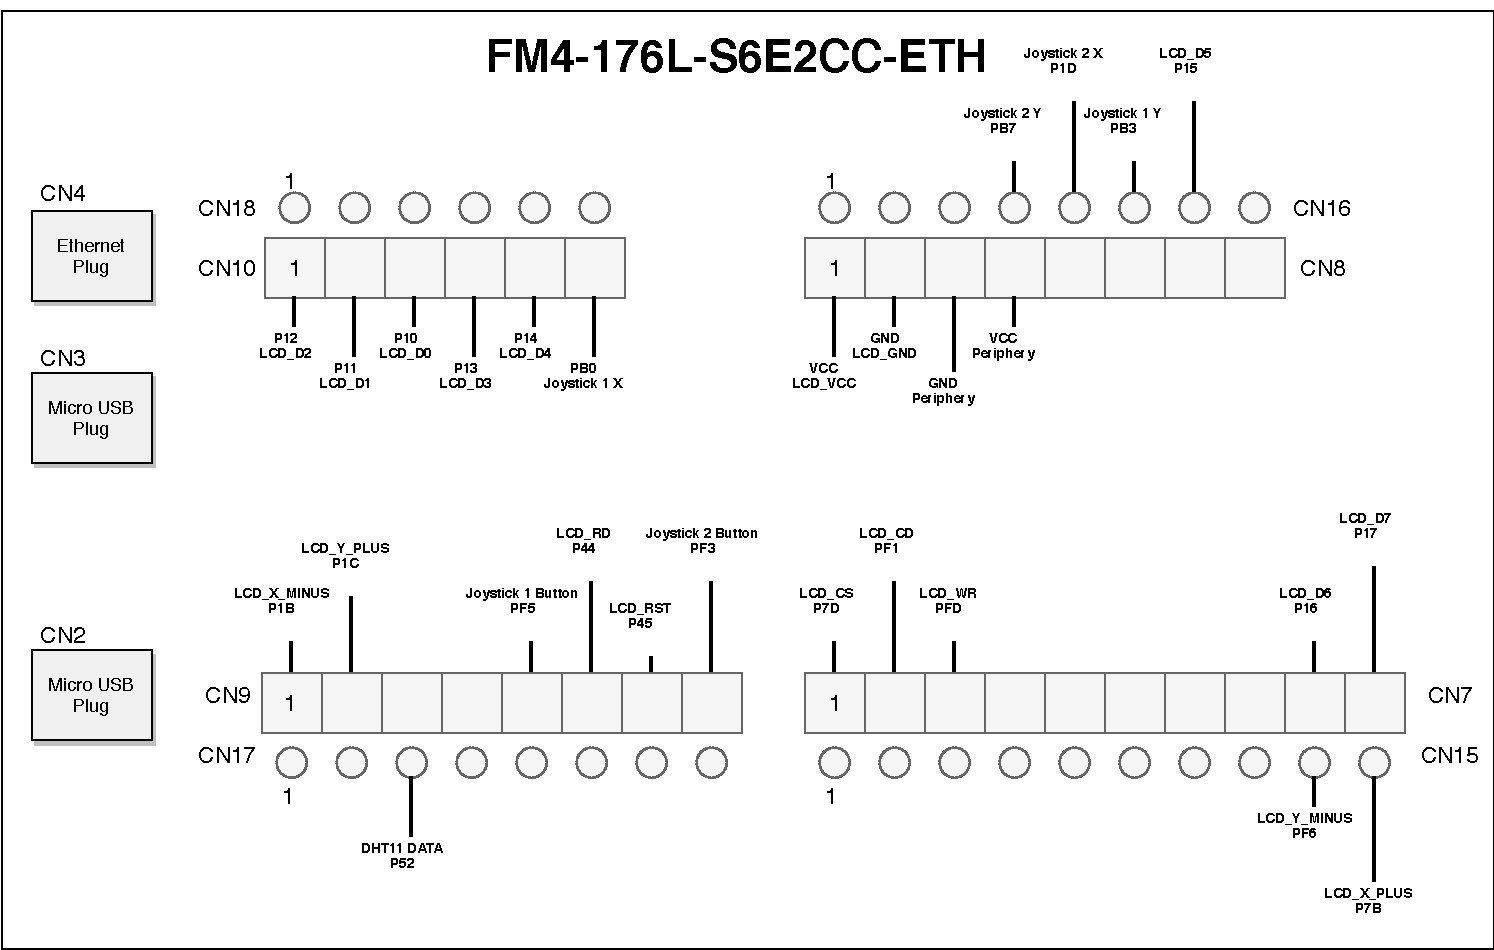
\includegraphics[width=0.7\textwidth]{./05_c/figures/cppp-wiring.pdf}
	\caption{Verkabelung des DHT11}
	\label{fig:cpppWiring}
\end{figure} 

\item 
In der Funktion \lstinline|readDHT11(uint8_t* humidity, uint8_t* temperature)| in der Datei \filename{dht11.c} wird zunächst eine Präambel vom DHT11 an den Microcontroller gesendet.
Hierdurch wird die Verbindung zwischen dem DHT11 und dem Microcontroller synchronisiert. 
Nach der Präambel beginnt der DHT11 40 Bits an den Microcontroller zu senden.
Abbildung \ref{fig:dht11Package} zeigt die Aufteilung der Bitgruppen.

Implementiere die fehlenden Stellen der Funktion \lstinline|readDHT11(uint8_t* humidity, uint8_t* temperature)|, indem du folgende Teilschritte umsetzt.
Nach der Präambel müssen zunächst die ankommenden Signale als 40~Bits interpretiert und in einem Array mit 5~Einträgen je 8~Bits gespeichert werden.
Lese mit \lstinline|Gpio1pin_Get(GPIO1PIN_P52)| den aktuellen Wert des digitalen Pins aus und entscheide entsprechend der folgenden Logik, ob es sich um eine 1 oder 0 handelt.
Ist der Pin länger als \SI{30}{\micro\second} auf \lstinline|HIGH| gesetzt $t_{HIGH} > \SI{30}{\micro\second}$, dann interpretiere dieses Signal als eine 1 und im umgekehrten Fall $t_{HIGH} < \SI{30}{\micro\second}$ als eine 0.
Nachdem alle 40 Bits empfangen wurden, bilde die Checksumme, welche die Summe der ersten 32 Bits darstellt. 
Ist der folgende Pseudocode erfüllt, dann ist die Übertragung der Daten erfolgreich gewesen.
%
\cpppInputListing{05_c/listings/dht11_checksum.c}
%
Beende die Methode  \lstinline|readDHT11readDHT11|, sofern die Checksumme nicht stimmt. 
Ist die Checksumme richtig, speichere die aktuelle Temperatur und Feuchtigkeit in den übergebenen Parametern \lstinline|humidity| und \lstinline|temperature|.
\begin{figure}[!htb]
	\centering
	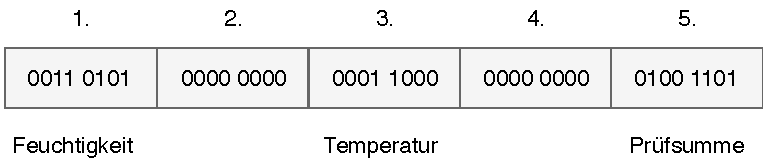
\includegraphics[width=0.7\textwidth]{./05_c/figures/dht11Bits.pdf}
	\caption{40 Bit Datenstruktur eines DHT11 Pakets}
	\label{fig:dht11Package}
\end{figure} 
\hints{
	\item Bei der Abfrage des Pins mithilfe von \lstinline|Gpio1pin_Get(GPIO1PIN_P52)|, kann es dazu kommen, dass fehlerhafte Signale dauerhaft auf \lstinline|HIGH| oder \lstinline|LOW| bleiben.
	Um diesen Fall zu filtern, verwende folgende Art der Abfrage.
	\cpppInputListing{05_c/listings/dht11.c}
	
	\item Um einen Delay auf dem Microcontroller ausführen, kannst du die Methode \lstinline|microDelay(uint32_t timeInMicroseconds)| verwenden. Zum Beispiel wird beim Aufruf  \lstinline|microDelay(20)| der Microcontroller \SI{20}{\micro\second} pausiert.
	
	\item Der DHT11 sendet immer seine Daten geordnet nach dem höchsten Bit, sodass der höchstwertigste Bit zuerst gesendet wird.
}

\item 
Nutze die Methoden \lstinline|writeTextln| und \lstinline|writeNumberOnDisplay| der Display-Library, um die Sensorenwerte auf dem Display auszugeben.

\hints{
	\item 
	Falls du die Funktionen \lstinline|writeTextln| und \lstinline|writeNumberOnDisplay| noch nicht implementiert hast, kannst du die Methoden der Musterlösung mit der Konkatenation des Suffix \lstinline|_s| nutzen (also \lstinline|writeTextln_s|).
}

\end{enumerate}